\documentclass{article}%
\usepackage[T1]{fontenc}%
\usepackage[utf8]{inputenc}%
\usepackage{lmodern}%
\usepackage{textcomp}%
\usepackage{lastpage}%
\usepackage[head=40pt,margin=0.5in,bottom=0.6in]{geometry}%
\usepackage{graphicx}%
%
\title{\textbf{Elecciones UC: denuncian polémico nombramiento de nueva comisión electoral}}%
\author{Cristian Briceñoi | @Cristianmbg92}%
\date{14/11/2018}%
%
\begin{document}%
\normalsize%
\maketitle%
\textbf{URL: }%
http://www.el{-}nacional.com/noticias/politica/elecciones{-}denuncian{-}polemico{-}nombramiento{-}nueva{-}comision{-}electoral\_259722\newline%
%
\textbf{Periodico: }%
EN, %
ID: %
259722, %
Seccion: %
Política\newline%
%
\textbf{Palabras Claves: }%
NO\_TIENE\newline%
%
\textbf{Derecho: }%
12, %
Otros Derechos: %
2.2, %
Sub Derechos: %
2.2.1.1\newline%
%
\textbf{EP: }%
NO\newline%
\newline%
%
\textbf{\textit{Los comicios estudiantiles se realizan luego~de las detenciones~del presidente saliente de la Federación de Centros Universitarios de la UC,~Iván Uzcátegui, y de~Ramón Bravo, director de comedores, que fueron privados de libertad por el Cuerpo de Investigaciones Científicas, Penales y Criminalísticas}}%
\newline%
\newline%
%
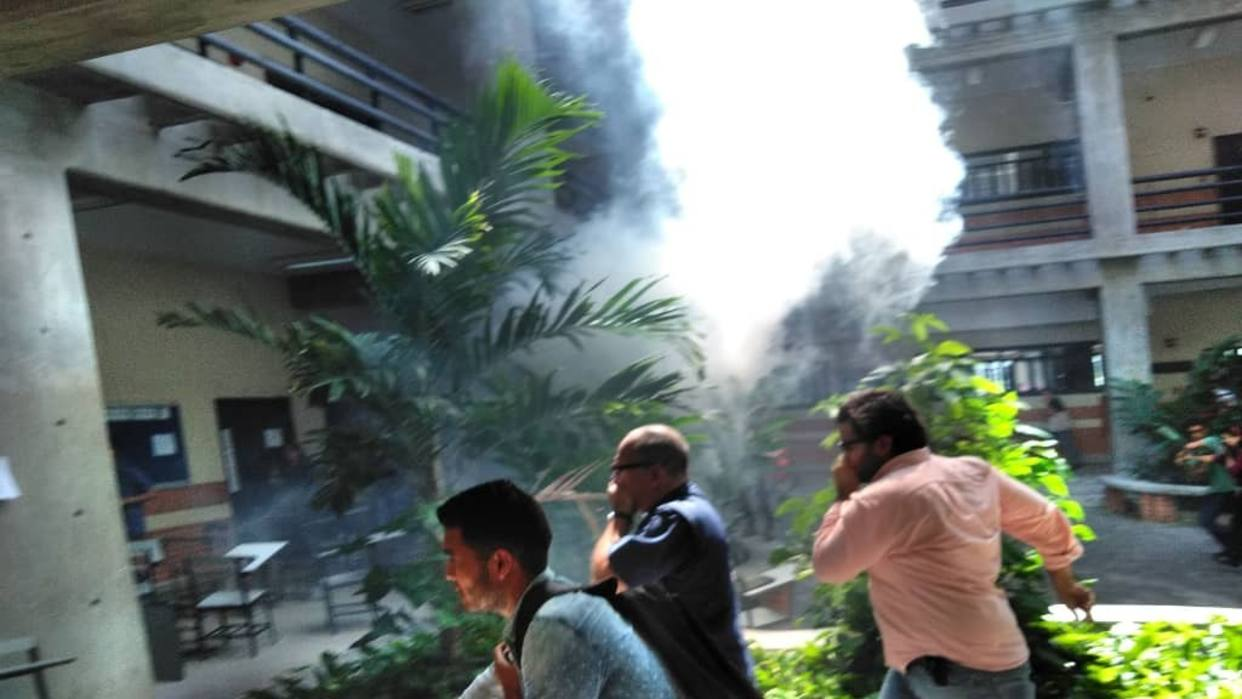
\includegraphics[width=300px]{166.jpg}%
\newline%
%
Pablo Aure, secretario de la Universidad de Carabobo, denunció este miércoles, día~ de elecciones estudiantiles en la entidad educativa autónoma, que en la noche de este martes se nombró una comisión electoral por parte de afectos al oficialismo y al gobernador del estado Carabobo, Rafael Lacava.%
\newline%
%
En principio el presidente de la comisión era el bachiller Eduardo León, y el nuevo presidente se llama Álvaro Londoño.%
\newline%
%
"Hubo una especie de 'golpe de estado' por gente afecta al gobernador que quiere constituir una comisión electoral paralela. Pero hay que dejar claro que la única comisión electoral estudiantil que existe es la presidida por el bachiller Eduardo León, y la comisión electoral presidida por el profesor José Manuel Ortega. Ellos están en sus funciones. Los afectos al gobernador nombraron un órgano que es írrito. No la reconocemos", explicó Aure en exclusiva a~El Nacional Web.%
\newline%
%
Eduardo León, presidente de la comisión, aseguró que a la candidata del oficialismo en la universidad se le entregaron todas las credenciales correspondientes.%
\newline%
%
"Quiero aclarar que les entregamos las credenciales, miembros de mesa, testigos, actas de apertura, y entregamos a la subcomisión. Cumplimos todos los pasos necesarios. Animo a todos a votar por la democracia", declaró el dirigente estudiantil.%
\newline%
%
Gabriel Cabrera, dirigente estudiantil, expresó para~El Nacional Web~que debido al "nombramiento" de la nueva comisión electoral no se habían abierto todas las mesas, porque las cajas tenían la firma del presidente de la comisión Eduardo León y no la de Álvaro Londoño.%
\newline%
%
"Lo nombraron en la madrugada y quisieron instalar mesas a nombre de ese presidente de comisión. Ya estamos restituyendo los centros originales con las cajas firmadas por León", explicó.%
\newline%
%
Hace poco se registró un ataque con una bomba lacrimógena en las instalaciones de la Universidad de Carabobo, mientras se desarrollaban los comicios. Hasta ese momento había afluencia, según Aure, de estudiantes universitarios ejerciendo su derecho a elegir sus autoridades universitarias.%
\newline%
%
Sairam Rivas, dirigente estudiantil, aseguró que entre grupos oficialistas apuntaron con armas de fuego a los testigos de mesa y se robaron cajas con votos.%
\newline%
%
"Le robaron el teléfono a varios de nosotros. Y golpearon a un montón de estudiantes", acotó.%
\newline%
%
Estas elecciones estudiantiles se realizan luego~de las detenciones~del presidente saliente de la Federación de Centros Universitarios de la UC,~Iván Uzcátegui, y de~Ramón Bravo, director de comedores, que fueron privados de libertad y acusados de peculado doloso y agavillamiento.%
\newline%
%
\end{document}